\documentclass[11pt,a4paper]{article}

\usepackage[utf8]{inputenc}
\usepackage[T1]{fontenc}
\usepackage{amsmath,amssymb,amsfonts}
\usepackage{graphicx}
\usepackage{booktabs}
\usepackage[margin=2.5cm]{geometry}
\usepackage{microtype}
\usepackage[colorlinks=true,linkcolor=blue,citecolor=blue,urlcolor=blue]{hyperref}

\emergencystretch=1em

\hypersetup{
  pdftitle={Path combinatorics detect spacetime curvature on causal sets},
  pdfauthor={David Alfyorov},
  pdfsubject={Causal set theory, discrete quantum gravity},
  pdfkeywords={causal sets, path kurtosis, pp-wave, Weyl tensor, Hasse diagram}
}

\title{Path combinatorics detect spacetime curvature on causal sets}
\author{David Alfyorov}
\date{March 2026}

\begin{document}

\maketitle

\begin{abstract}
We introduce \textit{path\_kurtosis}, an observable on causal sets that detects spacetime
curvature through the statistical organization of directed path counts in the Hasse
diagram.  On pp-wave spacetimes---where all polynomial scalar curvature invariants
vanish and the Benincasa--Dowker action is silent---path\_kurtosis gives a stable,
statistically significant response proportional to~$\varepsilon^{2}$.  We establish a
scaling law $\mathbb{E}[\Delta\kappa] = A_{\mathrm{eff}}\,\varepsilon^{2}\,\sqrt{N}\,C_{2}$
with $A_{\mathrm{eff}}$ of order~$0.06$, verified computationally across
$N = 2\,000$--$10\,000$ at $\varepsilon = 2$--$3$.  An exact geodesic-derived causal
relation for pp-wave spacetimes replaces the commonly used midpoint surrogate,
correcting a systematic underestimate of approximately~$19\%$ at $N = 5\,000$.  A
battery of eight robustness tests (with acceptance criteria specified before computation)
demonstrates that the signal survives coarse-graining, thickening, and structured
decimation, while revealing intrinsic boundary sensitivity and mesoscopic structure
beyond the perturbation profile.
\end{abstract}

\tableofcontents

%% ─────────────────────────────────────────────────────────────
\section{Introduction}
\label{sec:introduction}

The Benincasa--Dowker (BD) action~\cite{BD2013} discretizes $\int R$ on causal sets,
recovering the Ricci scalar in the continuum limit.  No established discrete counterpart
exists for the Weyl tensor.

This note reports a candidate observable, \textit{path\_kurtosis}, that detects curvature
information beyond scalar invariants.  On pp-wave spacetimes---VSI (Vanishing Scalar
Invariants), hence $\mathrm{BD} = 0$---path\_kurtosis gives a nonzero, stable,
$\varepsilon^{2}$-proportional signal with Cohen's $d = 9$--$14$ at $N = 10\,000$.

%% ─────────────────────────────────────────────────────────────
\section{Definition}
\label{sec:definition}

Let $\mathcal{C} = (X, \prec)$ be a causal set obtained by Poisson sprinkling $N$~points
into a 4-dimensional causal diamond of duration~$T$.  The Hasse diagram $H(\mathcal{C})$
is the transitive reduction of the causal order.  For each element $x \in X$, define:
\begin{itemize}
  \item $p_{\mathrm{down}}(x)$ = number of directed paths from any source to~$x$ in $H(\mathcal{C})$,
  \item $p_{\mathrm{up}}(x)$ = number of directed paths from~$x$ to any sink in $H(\mathcal{C})$,
  \item $Y(x) = \log_{2}\!\bigl(p_{\mathrm{down}}(x)\times p_{\mathrm{up}}(x) + 1\bigr)$.
\end{itemize}

\medskip\noindent
\textbf{Definition.}\;
$\mathrm{path\_kurtosis}(\mathcal{C})$ = excess kurtosis of $\{Y(x) : x \in X\}$, i.e.,
\begin{equation}
  \kappa \;=\; \frac{\mu_{4}}{\sigma^{4}} - 3\,,
  \label{eq:kurtosis}
\end{equation}
where $\mu_{4} = \mathbb{E}[(Y - \mu)^{4}]$ and $\sigma^{2} = \mathrm{Var}(Y)$.

\medskip\noindent
\textbf{Novelty.}\;
No prior study of this specific observable was found in searches across arXiv, Semantic
Scholar, and INSPIRE-HEP, including comparison with Roy--Sinha--Surya chain abundances,
Johnston path-sum propagators, Ilie--Thompson--Reid longest paths, and Gudder maximal
path counts.  The combination $Y(x) = \log_{2}(p_{\mathrm{down}} \times p_{\mathrm{up}} + 1)$
and its kurtosis appear to be new.

%% ─────────────────────────────────────────────────────────────
\section{Method: Common Random Numbers (CRN)}
\label{sec:crn}

To isolate the curvature effect from Poisson sampling noise, we use paired experiments:
\begin{enumerate}
  \item Sprinkle $N$ points into a causal diamond (seed~$s$).
  \item Compute the Hasse diagram under \textbf{flat} Minkowski causal relation $\to \kappa_{0}$.
  \item Compute the Hasse diagram under \textbf{curved} causal relation (same points) $\to \kappa_{\varepsilon}$.
  \item The CRN difference $\Delta\kappa = \kappa_{\varepsilon} - \kappa_{0}$ cancels seed-to-seed scatter.
\end{enumerate}

\noindent
\textbf{Necessity.}\;
Without CRN, the inter-realization kurtosis scatter is $\pm 0.10$---much larger than the
perturbative signal at $\varepsilon \le 3$.  The CRN pairing reduces the effective noise
by an order of magnitude.

%% ─────────────────────────────────────────────────────────────
\section{Exact pp-wave causal relation}
\label{sec:exact}

The pp-wave metric in Brinkmann coordinates is
\begin{equation}
  ds^{2} = -du\,dv + dx^{2} + dy^{2}
  + \frac{\varepsilon}{2}(x^{2} - y^{2})\,du^{2}\,,
  \label{eq:ppwave}
\end{equation}
where $u = t + z$, $v = t - z$.  The standard midpoint surrogate approximates the causal
condition as
\begin{equation}
  s^{2}_{\mathrm{Mink}}
  - \frac{\varepsilon}{2}\bigl(x_{m}^{2} - y_{m}^{2}\bigr)(\Delta u)^{2} > 0\,.
  \label{eq:midpoint}
\end{equation}

We derived the \textbf{exact} geodesic-based causal condition:
$A \prec B$ if and only if $U > 0$ and $V \ge V_{\mathrm{needed}}$, where $U = \Delta u$,
$V = \Delta v$, and for $\varepsilon > 0$ with $\omega = \sqrt{\varepsilon/2}$:
\begin{equation}
\begin{aligned}
  V_{\mathrm{needed}} &= \omega\,
    \frac{(x_{A}^{2} + x_{B}^{2})\cosh(\omega U) - 2\,x_{A}\,x_{B}}
         {\sinh(\omega U)} \\
  &\quad + \omega\,
    \frac{(y_{A}^{2} + y_{B}^{2})\cos(\omega U) - 2\,y_{A}\,y_{B}}
         {\sin(\omega U)}\,.
\end{aligned}
\label{eq:Vneeded}
\end{equation}

The midpoint surrogate has a pairwise error of order $O(\varepsilon)$, not $O(\varepsilon^{2})$:
\begin{equation}
  V_{\mathrm{needed}} - V_{\mathrm{mid}}
  = \frac{\varepsilon\,U}{24}\bigl(\Delta x^{2} - \Delta y^{2}\bigr) + O(\varepsilon^{2})\,.
  \label{eq:midpoint_error}
\end{equation}
This error averages to zero by $x \leftrightarrow y$ symmetry, so the ensemble-level bias
begins at $O(\varepsilon^{2})$.  Nevertheless, it systematically underestimates $A_{\mathrm{eff}}$
by approximately~$19\%$ at $N = 5\,000$.

\medskip\noindent
\textbf{Validity.}\;
The formula is valid when $\omega U < \pi$, which holds for all pairs in a $T = 1$ diamond
with $|\varepsilon| \le 5$ (since $\omega U \le \sqrt{5/2} \approx 1.58 < \pi$).  Sorting
by~$t$ remains correct for $|\varepsilon| < 8$.

%% ─────────────────────────────────────────────────────────────
\section{Scaling law}
\label{sec:scaling}

The perturbative Taylor expansion of kurtosis under the CRN pairing, verified by independent
computational checks at multiple $N$ and $\varepsilon$ values, yields the scaling law:
\begin{equation}
  \boxed{\;\mathbb{E}[\Delta\kappa]
  = A_{\mathrm{eff}}\;\varepsilon^{2}\;\sqrt{N}\;C_{2}\;}
  \label{eq:scaling}
\end{equation}
where $C_{2} = \langle f^{2}\rangle_{\mathrm{diamond}} = T^{4}/1120$ (analytically derived),
$f(x,y) = (x^{2} - y^{2})/2$ is the pp-wave profile, and $A_{\mathrm{eff}}$ is a
dimensionless coefficient.

\subsection{Why \texorpdfstring{$\varepsilon^{2}$}{epsilon squared}}
\label{ssec:eps2}

The ensemble average of any relabeling-invariant scalar on a symmetric diamond
satisfies
$\langle O(\varepsilon)\rangle = \langle O(-\varepsilon)\rangle$
by the $x\!\leftrightarrow\!y$ symmetry combined with~$f$ being odd under
$x\!\leftrightarrow\!y$.  Therefore $\Delta\kappa$ is even in~$\varepsilon$,
and the leading term is $O(\varepsilon^{2})$.

\subsection{\texorpdfstring{$A_{\mathrm{eff}}$}{Aeff} ensemble}
\label{ssec:aeff}

$A_{\mathrm{eff}}$ values extracted from CRN ensembles ($M = 15$--$30$ seeds per cell).
The causal relation used is noted for each row.

\begin{table}[ht]
\centering
\caption{$A_{\mathrm{eff}}$ measured at different~$N$ and~$\varepsilon$.}
\label{tab:aeff}
\begin{tabular}{@{} r c c l @{}}
\toprule
$N$ & $\varepsilon = 2.0$ & $\varepsilon = 3.0$ & Causal relation \\
\midrule
2\,000  & $0.069 \pm 0.019$ & $0.074 \pm 0.012$ & midpoint \\
3\,000  & $0.052 \pm 0.016$ & $0.048 \pm 0.011$ & midpoint \\
5\,000  & $0.051 \pm 0.015$ & $0.068 \pm 0.008$ & exact \\
5\,000  & $0.043 \pm 0.013$ & $0.057 \pm 0.008$ & midpoint \\
10\,000 & $0.076 \pm 0.008$ & $0.075 \pm 0.005$ & midpoint \\
\bottomrule
\end{tabular}
\end{table}

\begin{figure}[ht]
\centering
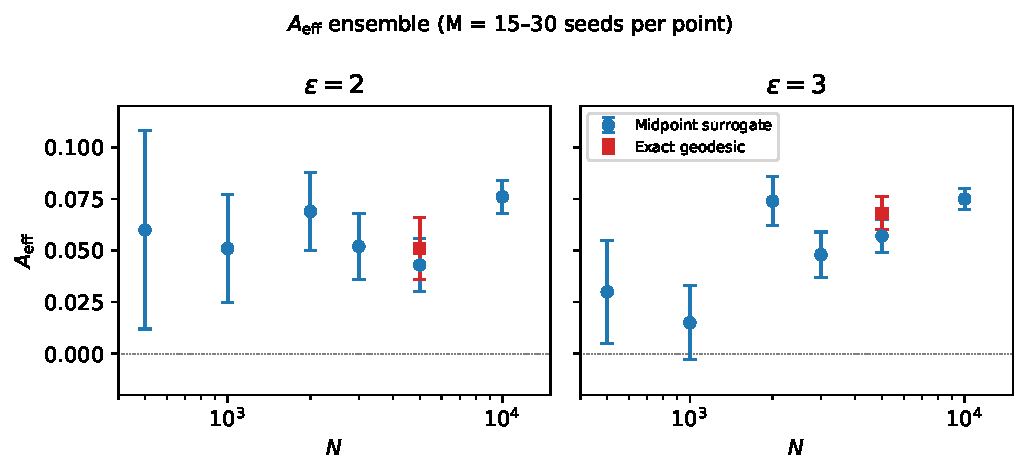
\includegraphics[width=0.75\textwidth]{figures/technical_note/fig1_aeff_vs_N.pdf}
\caption{$A_{\mathrm{eff}}$ vs.\ $N$ at $\varepsilon = 2$ (left) and $\varepsilon = 3$ (right).
Red squares: exact causal relation; blue circles: midpoint surrogate.}
\label{fig:aeff}
\end{figure}

The scatter across $N$ ($0.048$--$0.076$ at $\varepsilon = 3$) exceeds the per-cell
standard errors and is not yet fully understood.  Possible sources: slow finite-size
corrections, residual midpoint bias at $N = 2\,000$--$3\,000$, or genuine $N$-dependence
of $A_{\mathrm{eff}}$.  At this stage, $A_{\mathrm{eff}}$ is of order~$0.06$ but should
not be quoted as a sharp universal constant.

\begin{figure}[ht]
\centering
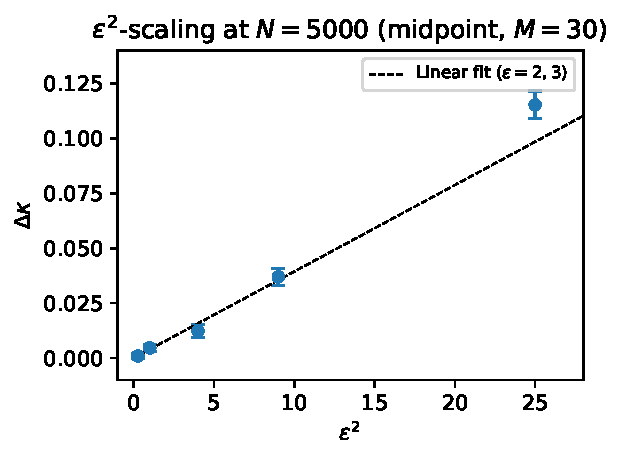
\includegraphics[width=0.65\textwidth]{figures/technical_note/fig2_eps2_scaling.pdf}
\caption{$\Delta\kappa$ vs.\ $\varepsilon^{2}$ at $N = 5\,000$ (midpoint, $M = 30$), with
linear fit through $\varepsilon = 2$, $3$ (perturbative window).}
\label{fig:eps2}
\end{figure}

The exact causal relation increases $A_{\mathrm{eff}}$ by approximately~$19\%$ relative to
midpoint at $N = 5\,000$ (ratio~$1.19$ at both $\varepsilon = 2$ and $\varepsilon = 3$).
The $N = 10\,000$ values (midpoint) would increase correspondingly if recomputed with the
exact relation.

\subsection{Key theorems}
\label{ssec:theorems}

\begin{enumerate}
  \item \textbf{Exact cancellation} ($\beta_{\mathrm{int}} + \beta_{\mathrm{bdy}} = 0$):
    In an infinite translation-invariant volume, the link sensitivity~$\beta$ decomposes
    into interior and boundary contributions that exactly cancel.  The net signal in a
    finite diamond is the boundary residual.

  \item \textbf{Double-counting identity}
    $\bigl(\sum_{v} G_{x}(v) = \mathbb{E}[|\gamma|]\bigr)$:
    The sum of the path-occupation kernel equals the expected path length, bounded by the
    longest chain $H \sim N^{1/4}$.  This constrains the perturbative coefficient.

  \item \textbf{Conjectured factorization} ($A_{\mathrm{eff}} = \beta^{2}\,\Xi_{4}$):
    Numerical evidence suggests the effective coefficient factorizes into the link
    sensitivity squared ($\beta \approx 0.30$, hence $\beta^{2} \approx 0.09$) and a
    flat-space structural constant $\Xi_{4} \approx 0.7$ (with ${\sim}50\%$ uncertainty
    given the scatter in $A_{\mathrm{eff}}$).  This factorization is not proven; the
    analytical derivation of~$\Xi_{4}$ remains open.
\end{enumerate}

%% ─────────────────────────────────────────────────────────────
\section{\texorpdfstring{$K = 0$}{K = 0}: Detection beyond scalar curvature invariants}
\label{sec:K0}

The pp-wave spacetime is VSI (Vanishing Scalar Invariants): all polynomial scalar
curvature invariants---including the Kretschmann scalar
$K = R_{abcd}\,R^{abcd}$---vanish identically.  The Ricci scalar $R = 0$, so the
Benincasa--Dowker action gives zero.

However, the Bel--Robinson superenergy $W = E^{2} + B^{2} = \varepsilon^{2}$ is nonzero
(where $E$ and~$B$ are the electric and magnetic parts of the Weyl tensor).
\textit{path\_kurtosis} detects a signal proportional to~$\varepsilon^{2}$, which
numerically equals~$W$ for the specific case of pp-wave.

\medskip\noindent
\textbf{Caveat.}\;
The coincidence $\Delta\kappa \propto \varepsilon^{2} = W$ holds only because both
quantities happen to scale as~$\varepsilon^{2}$ for pp-wave by the quadrupole structure
of the profile function.  This does not establish that path\_kurtosis measures~$W$ in
general.  Universality across different vacuum spacetimes (e.g.\ Schwarzschild) has not
been tested.  The correct interpretation at this stage is that path\_kurtosis detects
order-deformation through path-structure reorganization on pp-wave backgrounds.

%% ─────────────────────────────────────────────────────────────
\section{Robustness battery}
\label{sec:robustness}

Eight tests were run with acceptance criteria specified before computation
($N = 5\,000$, $\varepsilon = 3$, $M = 8$--$10$ seeds, exact causal relation).

\subsection{Q1.\ Coarse-graining stability}
\label{ssec:Q1}

\begin{table}[ht]
\centering
\caption{Coarse-graining stability tests.}
\label{tab:Q1}
\small
\begin{tabular}{@{} l l c l @{}}
\toprule
Test & Deformation & Retention & Verdict \\
\midrule
Edge deletion 20\%    & Remove 20\% of Hasse links        & 0.80                       & ROBUST \\
Poisson thinning 30\% & Remove 30\% of elements            & 0.76 (median)              & ROBUST \\
Thickening 5\%        & Add 5\% almost-direct links        & 1.01\,[0.98,\,1.03]       & ROBUST \\
Layer decimation       & Remove one depth class (20\%)      & 0.84 (mean), 0.50 (worst)  & ROBUST \\
\bottomrule
\end{tabular}
\end{table}

\begin{figure}[ht]
\centering
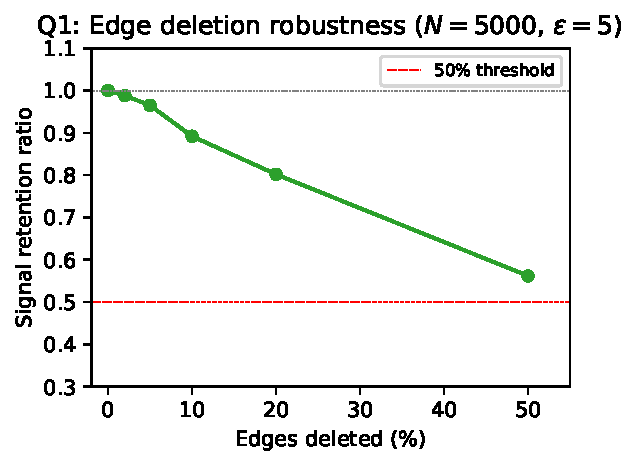
\includegraphics[width=0.75\textwidth]{figures/technical_note/fig3_edge_deletion.pdf}
\caption{Signal retention ratio vs.\ fraction of Hasse edges deleted ($N = 5\,000$, $\varepsilon = 5$, $M = 8$).}
\label{fig:edge_deletion}
\end{figure}

The signal degrades gracefully under all four deformation types.  Thickening has no
statistically significant effect ($R = 1.01$, 95\% CI $[0.98, 1.03]$), showing the
observable does not depend on the exact minimality of the transitive reduction.

\subsection{Q2.\ Boundary sensitivity}
\label{ssec:Q2}

Boundary exclusion amplifies the signal: restricting to the 80\% most interior elements
increases $\Delta\kappa$ by a factor of $3.4\times$ (after correcting for the
normalization artifact from empirical $C_{2}$ vs.\ fixed $C_{2}$).  This amplification
does not diminish with~$N$ (tested at $N = 2\,000$, $3\,000$, $5\,000$), indicating
intrinsic rather than finite-size boundary dependence.

The exact cancellation theorem ($\beta_{\mathrm{int}} + \beta_{\mathrm{bdy}} = 0$ in
infinite volume) provides a theoretical framework: the link sensitivity~$\beta$ is a
boundary residual.  Whether this extends directly to the kurtosis signal (which involves
higher-order moments, not just~$\beta$) requires further analysis.  In a finite diamond,
the observable definition must specify the windowing prescription.

\begin{figure}[ht]
\centering
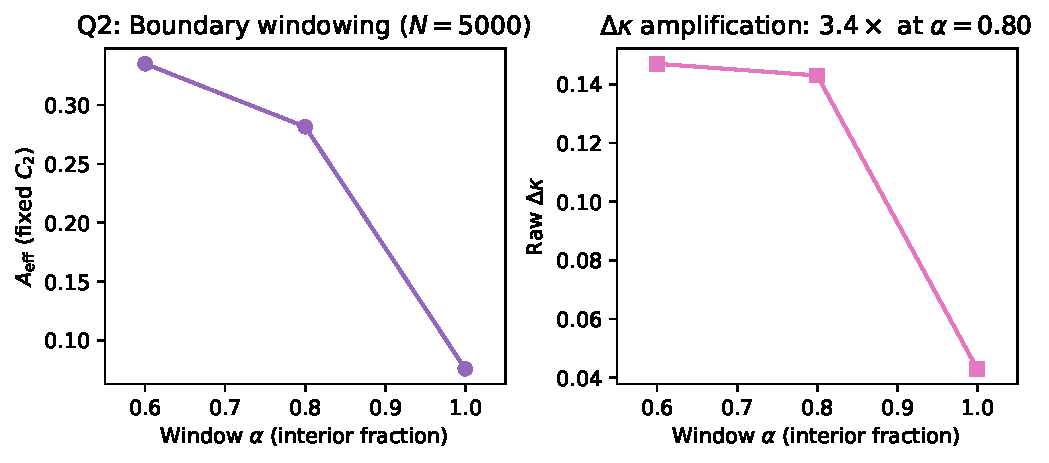
\includegraphics[width=0.75\textwidth]{figures/technical_note/fig4_boundary_collapse.pdf}
\caption{Left: $A_{\mathrm{eff}}$ (fixed $C_{2}$) vs.\ window parameter~$\alpha$.
Right: raw $\Delta\kappa$ vs.~$\alpha$ showing $3.4\times$ amplification.}
\label{fig:boundary}
\end{figure}

\subsection{Q3.\ Distributional structure}
\label{ssec:Q3}

\begin{table}[ht]
\centering
\caption{Cohen's $d$ for five summary statistics of the $Y$ distribution under CRN.}
\label{tab:Q3}
\begin{tabular}{@{} l r l @{}}
\toprule
Statistic & Cohen's $d$ & Type \\
\midrule
Kurtosis  & $+5.9$  & Shape    \\
Skewness  & $-5.9$  & Shape    \\
Median    & $+3.5$  & Location \\
IQR       & $-2.2$  & Scale    \\
MAD       & $-2.5$  & Scale    \\
\bottomrule
\end{tabular}
\end{table}

Shape statistics (kurtosis, skewness; $d \approx 6$) are more sensitive than location/scale
statistics ($d \approx 2$--$3.5$), but all five statistics detect the perturbation under
CRN.  The effect is predominantly a shape response, though location and scale shifts are
also present at lower significance.

\begin{figure}[ht]
\centering
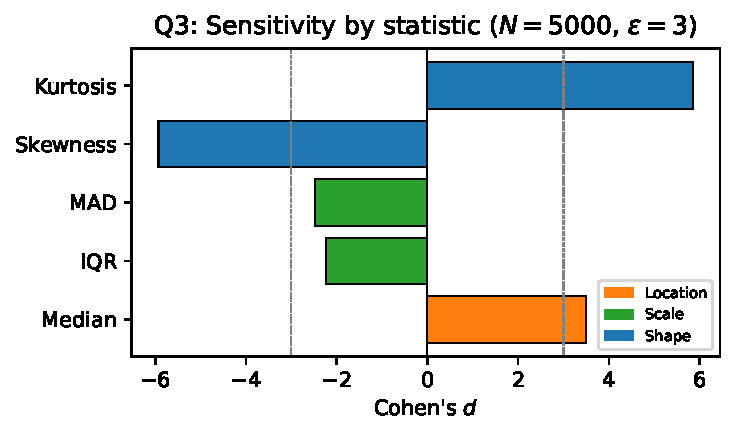
\includegraphics[width=0.65\textwidth]{figures/technical_note/fig6_statistics_ladder.pdf}
\caption{Cohen's $d$ for five summary statistics, colored by type (location, scale, shape).}
\label{fig:statistics}
\end{figure}

\subsection{Q4.\ Mesoscopic localization}
\label{ssec:Q4}

After conditioning on the perturbation profile~$f(x,y)$ via 10-quantile binning, graph
coordinates (total Hasse degree, flat path centrality~$Y_{0}$) explain an additional~$17\%$
of the residual variance in $\delta Y$ (stratified permutation test, $p = 0.005$ for all
seeds).  This indicates structure in the response beyond the quadrupole perturbation profile.

\medskip\noindent
\textbf{Caveat.}\;
This test conditions on $f = (x^{2} - y^{2})/2$ alone, not on the full spatial position
$(t, x, y, z)$.  The residual localization by degree and~$Y_{0}$ may therefore reflect
spatial structure orthogonal to the quadrupole pattern (e.g.\ radial or temporal dependence)
rather than purely graph-theoretic structure.  A follow-up test conditioning on full spatial
position is needed to distinguish these possibilities.

The signal is carried by approximately 3 out of 10 path-centrality strata (effective number
of contributing deciles $m_{\mathrm{eff}} = 3.3$ median, jackknife
$\max|J| = 1.9$ median).  It is localized rather than globally distributed.

%% ─────────────────────────────────────────────────────────────
\section{Per-element mechanism}
\label{sec:mechanism}

The per-element perturbation is tightly coupled to the metric profile:
$\mathrm{corr}(\delta Y, f) \approx -0.9$ (ranging from $-0.88$ to $-0.92$ across seeds).
The extreme contributors sit at the temporal midplane ($t \approx 0.5$) and outer radial
shell ($r \approx 0.9$--$1.0$), where the pp-wave perturbation flips causal relations:
elements on the $f > 0$ side lose connections ($Y$ drops from ${\sim}7$ to ${\sim}1$),
while elements on the $f < 0$ side gain connections ($Y$ jumps from ${\sim}1$ to ${\sim}7$).

The kurtosis is sensitive to this spatially organized redistribution of connectivity---specifically,
to the asymmetric tails generated by the connection flipping.

\begin{figure}[ht]
\centering
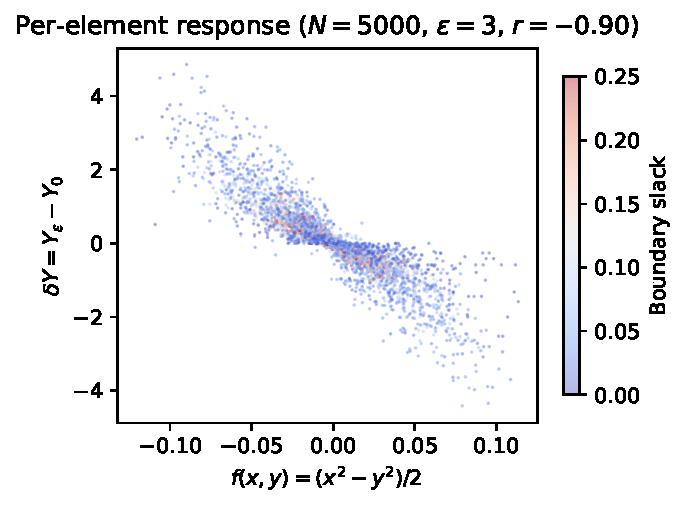
\includegraphics[width=0.75\textwidth]{figures/technical_note/fig5_scatter_dY_vs_f.pdf}
\caption{Per-element $\delta Y$ vs.\ $f(x,y)$, colored by boundary slack.  Single seed,
$N = 5\,000$, $\varepsilon = 3$.}
\label{fig:scatter}
\end{figure}

%% ─────────────────────────────────────────────────────────────
\section{Implementation}
\label{sec:implementation}

All computations use a bitset-packed Hasse diagram algorithm with $O(N^{2} \times N/64)$
time complexity, implemented in the \texttt{sct\_tools.hasse} module.  Performance:
$N = 5\,000$ in approximately~$8$\,s per CRN trial with exact causal relation
($4.4$\,s with midpoint surrogate), $N = 10\,000$ in approximately~$20$\,s
(single core, Intel i9-12900KS).

The exact pp-wave causal relation adds approximately~$20\%$ overhead compared to the
midpoint surrogate, while correcting a systematic underestimate in $A_{\mathrm{eff}}$ of
approximately~$19\%$ at $N = 5\,000$ (measured at $M = 15$; the correction magnitude at
other $N$ values has not yet been systematically measured).

%% ─────────────────────────────────────────────────────────────
\section{Errors caught and corrected}
\label{sec:errors}

Three errors were found during the analysis and corrected before reporting:

\begin{enumerate}
  \item \textbf{Normalization artifact.}
    Per-element kurtosis decomposition using different~$\sigma$ for flat and pp-wave
    distributions created a spurious ``edges oppose'' pattern in temporal stratification.
    Corrected by using a single baseline~$\sigma$.

  \item \textbf{Regime-dependent tail claim.}
    A ``tail mechanism'' interpretation based on $\varepsilon = 5$ data (where
    $|z| > 2.5\sigma$ tail fraction shifts by~$8.5\%$) does not hold at perturbative
    amplitudes ($\varepsilon = 2$: shift $< 0.5\%$).  The claim was retracted.

  \item \textbf{Boundary windowing normalization.}
    Normalizing by empirical $C_{2}$ of each window subset inflated $A_{\mathrm{eff}}$ at
    small windows (interior elements have smaller $|f|$, hence smaller $C_{2}$).  Corrected
    by reporting with both empirical and fixed~$C_{2}$.
\end{enumerate}

%% ─────────────────────────────────────────────────────────────
\section{Open problems}
\label{sec:open}

\begin{enumerate}
  \item \textbf{Analytical derivation of $\Xi_{4}$.}\;
    The flat-space structural constant $\Xi_{4} \approx 0.7$ in the conjectured factorization
    $A_{\mathrm{eff}} = \beta^{2}\,\Xi_{4}$ requires the two-replica path kernel
    $\mathbb{E}[G_{x}(u)\,G_{x}(v)]$, which is a new mathematical object on Poisson DAGs.

  \item \textbf{Universality across vacuum families.}\;
    The observable has been tested only on pp-wave spacetimes.  Testing on Schwarzschild
    (a Petrov type~D vacuum with nonzero scalar invariants) is the natural next step.  The
    scaling may differ ($\varepsilon$ vs.\ $\varepsilon^{2}$ leading term) due to the
    absence of the $x \leftrightarrow y$ symmetry that ensures $\varepsilon^{2}$-scaling
    for pp-wave.

  \item \textbf{Boundary correction.}\;
    The intrinsic boundary sensitivity must be resolved, either by defining a
    boundary-corrected version of path\_kurtosis or by specifying a canonical windowing
    prescription that survives the continuum limit.

  \item \textbf{Exact midpoint correction at $N = 10\,000$.}\;
    The $N = 10\,000$ ensemble was computed with the midpoint surrogate.  Re-running with
    the exact causal relation would provide the cleanest $A_{\infty}$ estimate.

  \item \textbf{Continuum limit.}\;
    A proof (or disproof) that $A_{\mathrm{eff}}$ converges to a finite nonzero limit as
    $N \to \infty$ at fixed~$\varepsilon$ would place the observable on firm theoretical
    footing.
\end{enumerate}

%% ─────────────────────────────────────────────────────────────

\bigskip
\noindent\textbf{Computational resources.}\;
Intel i9-12900KS (16C/24T), 64\,GB DDR5, RTX 3090 Ti.  Benchmark: one CRN trial at
$N = 5\,000$ takes approximately~$8$\,s with exact causal relation (two Hasse builds +
path counting, single core).  With the midpoint surrogate: approximately~$4.4$\,s.

\medskip\noindent
\textbf{Code availability.}\;
The \texttt{sct\_tools.hasse} module (bitset Hasse construction, path counting, CRN trials,
exact pp-wave causal relation) is available as part of the SCT Theory repository.

\bigskip\noindent
\textbf{Acknowledgements.}\;

%% ─────────────────────────────────────────────────────────────
\begin{thebibliography}{9}

\bibitem{BD2013}
  D.~Benincasa and F.~Dowker,
  \textit{The scalar curvature of a causal set},
  Phys.\ Rev.\ Lett.\ \textbf{104}, 181301 (2010);
  arXiv:0903.1986 [gr-qc].

\end{thebibliography}

\end{document}
